
\documentclass[twoside,twocolumn]{article}

\usepackage{blindtext} % Package to generate dummy text throughout this template 

\usepackage[sc]{mathpazo} % Use the Palatino font
\usepackage[T1]{fontenc} % Use 8-bit encoding that has 256 glyphs
\linespread{1.05} % Line spacing - Palatino needs more space between lines
\usepackage{microtype} % Slightly tweak font spacing for aesthetics
\usepackage{float}
\usepackage[english]{babel} % Language hyphenation and typographical rules

\usepackage{graphicx}
\usepackage[hmarginratio=1:1,top=32mm,columnsep=15pt]{geometry} % Document margins
\usepackage[hang, small,labelfont=bf,up,textfont=it,up]{caption} % Custom captions under/above floats in tables or figures
\usepackage{booktabs} % Horizontal rules in tables

\usepackage{lettrine} % The lettrine is the first enlarged letter at the beginning of the text

\usepackage{enumitem} % Customized lists
\setlist[itemize]{noitemsep} % Make itemize lists more compact

\usepackage{abstract} % Allows abstract customization
\renewcommand{\abstractnamefont}{\normalfont\bfseries} % Set the "Abstract" text to bold
\renewcommand{\abstracttextfont}{\normalfont\small\itshape} % Set the abstract itself to small italic text

\usepackage{titlesec} % Allows customization of titles
\renewcommand\thesection{\Roman{section}} % Roman numerals for the sections
\renewcommand\thesubsection{\roman{subsection}} % roman numerals for subsections
\titleformat{\section}[block]{\large\scshape\centering}{\thesection.}{1em}{} % Change the look of the section titles
\titleformat{\subsection}[block]{\large}{\thesubsection.}{1em}{} % Change the look of the section titles

\usepackage{fancyhdr} % Headers and footers
\pagestyle{fancy} % All pages have headers and footers
\fancyhead{} % Blank out the default header
\fancyfoot{} % Blank out the default footer
\fancyhead[C]{Joel Stuart $\bullet$ September 2016 $\bullet$ COSC3500 $\bullet$ Project Milestone Two} % Custom header text
\fancyfoot[RO,LE]{\thepage} % Custom footer text

\usepackage{titling} % Customizing the title section

\usepackage{hyperref} % For hyperlinks in the PDF

%----------------------------------------------------------------------------------------
%	TITLE SECTION
%----------------------------------------------------------------------------------------

\setlength{\droptitle}{-4\baselineskip} % Move the title up

\pretitle{\begin{center}\Huge\bfseries} % Article title formatting
	\posttitle{\end{center}} % Article title closing formatting
\title{Elastic Collisions in Two Dimensions COSC3500 Project Milestone 2} % Article title
\author{%
	\textsc{Joel Stuart - 43203714} \\[1ex] % Your name
	\normalsize University of Queensland \\ % Your institution
	\normalsize \href{mailto:joel.stuart@uq.net.au}{joel.stuart@uq.net.au} % Your email address
	%\and % Uncomment if 2 authors are required, duplicate these 4 lines if more
	%\textsc{Jane Smith}\thanks{Corresponding author} \\[1ex] % Second author's name
	%\normalsize University of Utah \\ % Second author's institution
	%\normalsize \href{mailto:jane@smith.com}{jane@smith.com} % Second author's email address
}
\date{\today} % Leave empty to omit a date
\renewcommand{\maketitlehookd}{%
	\begin{abstract}
		\noindent This report investigates a parallel implementation of a multi-bodied simulation of elastic collisions in two dimensions. It details the parallelisation and optimisation strategies used in this implementation. It also discusses the performance of the implementation at varying problem sizes and details the verifcation methods.
	\end{abstract}
}

%----------------------------------------------------------------------------------------

\begin{document}
	
	% Print the title
	\maketitle
	
	\section{Introduction}
	
	\lettrine[nindent=0em,lines=3]{T}o implement a physics simulation such as shooting an object into an asteroid belt or shooting one pool ball at another, the physics of a collision between objects needs to be modelled. \newline
	
	For this report, the scope of the problem has been reduced to the two dimensional plane and to elastic collisions. An elastic collision is a collision between two bodies where the total kinetic energy of the two objects before the encounter is equal to the total kinetic energy after the encounter. \newline 
	
	The simulation of object collisions is applicable to many areas of science including (but by no means limited to) describing the collision of atoms (Rutherford backscattering) and various physics problems.\newline 
	
	This report wil investigate a parallel implementation of a multi-bodied simulation of elastic collisions in two dimensions.\newline
	
	 It will detail the parallelisation and optimisation strategies used. It will discuss the performance of the implementation as well as the verification methods used.
	
	
	%------------------------------------------------
	\section{Parallelisation and Optimisation Strategies}
	As the time portion of this problem is inherently sequential, parallelisation over the time domain is outside the scope of this project. \newline 
	Thus, the parallelisation methods used in this project can be broken down into the following (concerning the parallelisation of objects within each timestep):
	
	\begin{itemize}
		\item OpenMP parallelisation for the initialisation of all objects (including random number generation)
		\item OpenMP parallelisation for the propogation of objects forward in time
		\item MPI parallelisation to calculate collisions between every unique object pair (through domain decomposition of the list of objects)
	\end{itemize}
	
	The overall runtime speedup of the OpenMP parallelisation optimisations was expected to be minor compared to speedups through parallelisation of the collision detection and simulation routines. \newline
	This was suggested by initial profiling of the serial implementation and Big-Oh analysis of the collision detection and simulations routines (due to nested for loops with costly mathematical operations and numerous array operations within). \newline
	
	To support MPI parallisation, several adjustments needed to be implemented:
	
		\begin{itemize}
			\item Domain decomposition of the object list to facilitate parallel collision detection and simulation
			\item Maintaining a buffer of colliding object pairs which lie outside of the local domain of each thread to avoid concurrency conflicts.  \newline
			This buffer was then used to serially calculate the collisions after the local collisions had been gathered into the global object list. 
		\end{itemize}
		

	%------------------------------------------------
	
		
	%------------------------------------------------
	
	\section{Parallel Performance}
	Results of performance scaling with problem size can be seen in Table 1 and Figure 2. \newline
	
	\begin{table}[H]
		\caption{Average performance over problem size}
		\centering
		\begin{tabular}{llr}
			\toprule
			\multicolumn{2}{c}{Problem size} \\
			\cmidrule(r){1-2}
			Num. Objects & Parallelisation & Run Time (s) \\
			\midrule
			200 & Milestone 1 Code & $0.41s$ \\
			200 & Milestone 2 Code (serial) & $0.67s$ \\
			200 & OpenMP (2) & $0.61s$ \\
			200 & OpenMP (4) & $0.61s$ \\
			200 & OpenMP (8) & $0.61s$ \\
			200 & OpenMP (2) MPI (2) & $0.59s$ \\
			200 & OpenMP (2) MPI (4) & $0.59s$ \\
			\midrule
			2000 & Milestone 1 Code & $8.8s$ \\
			2000 & Milestone 2 Code (serial) & $8.6s$ \\
			2000 & OpenMP (2) & $6.8s$ \\
			2000 & OpenMP (4) & $6.8s$ \\
			2000 & OpenMP (8) & $6.8s$ \\
			2000 & OpenMP (2) MPI (2) & $4.3s$ \\
			2000 & OpenMP (2) MPI (4) & $2.6s$ \\
			\midrule
			5000 & Milestone 1 Code & $50s$ \\
			5000 & Milestone 2 Code (serial) & $37s$ \\
			5000 & OpenMP (2) & $37s$ \\
			5000 & OpenMP (2) MPI (2) & $24.3s$ \\
			5000 & OpenMP (2) MPI (4) & $11.1s$ \\

			\bottomrule
		\end{tabular}
	\end{table}	
	
		\begin{figure*}
			\caption{Average Run Time vs Number of Objects Graph}
			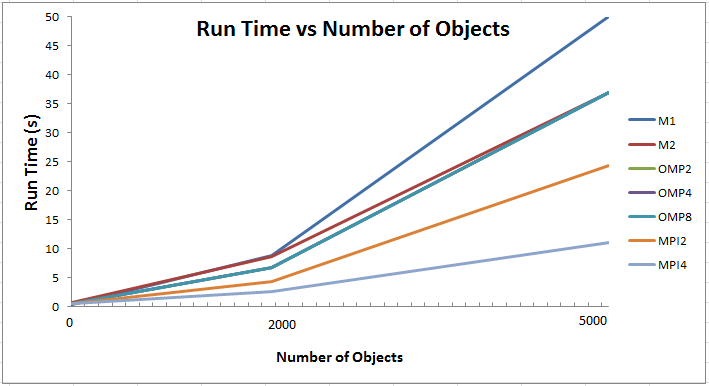
\includegraphics[scale=.9]{graph.png}
		\end{figure*}
	\subsection{OpenMP Analysis}
	As suggested earlier in the report, the effectiveness of the OpenMP parallelisation in terms of overall computation speedup was minor due to comparitive cost of the collision detection and simulation. For moderately sized problems, OpenMP offered a slight improvement in run time.
	
	\subsection{MPI Analysis}
	The most effective speedups offered were by the MPI parallelisations, which resulted in significant speedups with large numbers of objects. 
	
	
	\newpage
	\section{Verification}
	
	To verify the small scale implementation, a visualiser was built in Java which plots all of the objects within 2d space and animates over the time steps, using the output file of the C program. This visualisation is a means to verify the implementation at smaller problem sizes. \newline
	
	The visualiser is bundled with the report in both .jar file and executable form. This is bundled on the repository along with the source code also. \newline
	
	\begin{figure}
		\caption{Java Visualiser Demonstration}
		\includegraphics[scale=.4]{picvis.png}
	\end{figure}
	
	The bundled visualiser is able to visualise objects in the domain and range of [-200, 200]. It is worth noting that the frame rate of the visualiser suffers with large problem sizes (greater than 500 objects). \newline
	
	Further verification of the implementation can be achieved by checking individual objects in the output file. For the next milestone, an individual output file will be made for each thread, so that each thread's results (as well as the combined thread results) can be visualised. \newline
	
	The following steps have been taken to verify the implementation: \newline
	
	\begin{itemize}
		\item Check functionality at small object and time step values
		\item Print all position and velocity values into a file and manually check physics.
		\item Print all collisions and related object information into file upon occurance
	\end{itemize}
	
	
	\section{Relation to Initial Scientific Task}
	
	The previous sections have covered the main progress of the project - moving into the large scale domain thanks to parallelisation and 
	the addition of the visualisation. \newline
	
	Concerning the initially proposed scientific task (i.e. a simulation of phyiscal collisions between 2D objects such as asteroids of pool balls), the project has begun to demonstrate these simulation capabilities. \newline
	
	With the next milestone, the author hopes to dial up these simulations and visualisation to address the initial scientific task more directly. 
	%----------------------------------------------------------------------------------------
	%	REFERENCE LIST
	%----------------------------------------------------------------------------------------
	
	
	%----------------------------------------------------------------------------------------
	
\end{document}\documentclass{article}
